\documentclass[12pt]{article}
\usepackage{amsmath}
\usepackage{graphicx}
\usepackage{caption}
\usepackage{subcaption}
\usepackage[margin=1in]{geometry}
\usepackage{float}
\usepackage{multicol}
\usepackage{multirow}
\usepackage[table,xcdraw]{xcolor}
\usepackage[]{algorithm2e}
\usepackage{amssymb}


\title{\textbf{COMP 540 Homework 2}}

\author{Tony Ren, Hanyang (Quentin) Li }

\begin{document}
\maketitle

\section*{Problem 1}
\subsection*{Problem 1.1}
\begin{equation} \label{eq1}
\begin{split}
\frac{\partial g(z)}{\partial z}  & =\frac{\partial }{\partial z}(1+e^{-z})^{-1}  \\
 & =\frac{\partial (1+e^{-z})^{-1}}{\partial (1+e^{-z})} \cdot \frac{\partial (1+e^{-z})}{\partial z}\\
 & =-(1+e^{-z})^{-2} \cdot (-e^{-z})\\
 & =\frac{e^{-z}}{(1+e^{-z})^{2}} 
\end{split}
\end{equation}
Since $g(z) = \frac{1}{1+e^{-z}}$ and $1-g(z) = \frac{e^{-z}}{1+e^{-z}}$, then 
$$g(z)(1-g(z)) = \frac{e^{-z}}{(1+e^{-z})^{2}}$$
Therefore,
$$\frac{\partial g(z)}{\partial z}  = g(z)(1-g(z)) $$

\subsection*{Problem 1.2}
\begin{equation} \label{eq2}
\begin{split}
NLL(\theta)  & =-logP(D|\theta) \\
 & =-\sum\limits_{i=1}^m y^{(i)}log[h_\theta (x^{(i)})] + (1-y^{(i)}) log[1 - h_\theta (x^{(i)})] 
\end{split}
\end{equation}
\begin{equation} \label{eq3}
\begin{split}
\frac{\partial }{\partial \theta} NLL(\theta)  & =  -\frac{\partial }{\partial \theta} \sum\limits_{i=1}^m y^{(i)}log[ g(\theta ^{T} x^{(i)})] - \frac{\partial }{\partial \theta} \sum\limits_{i=1}^m (1-y^{(i)} ) log[1 - g(\theta ^{T} x^{(i)}] \\
 &= -\sum\limits_{i=1}^m [\frac{y^{i}}{g(\theta ^{T} x^{(i)})} \cdot \frac{\partial }{\partial \theta} g(\theta ^{T} x^{(i)}) + \frac{1-y^{(1)}}{1-g(\theta ^{T} x^{(i)}} \cdot(-1) \frac{\partial }{\partial \theta}  g(\theta ^{T} x^{(i)})]\\
  &=-\sum\limits_{i=1}^m [[\frac{y^{i}}{g(\theta ^{T} x^{(i)})} - \frac{1-y^{i}}{1-g(\theta ^{T} x^{(i)})}] \cdot \frac{\partial }{\partial \theta}  g(\theta ^{T} x^{(i)})]\\
  &=-\sum\limits_{i=1}^m [[\frac{y^{i}}{g(\theta ^{T} x^{(i)})} - \frac{1-y^{i}}{1-g(\theta ^{T} x^{(i)})}] \cdot  g(\theta ^{T} x^{(i)}) \cdot (1-g(\theta ^{T} x^{(i)})) \cdot x^{(i)}]\\
  &= -\sum\limits_{i=1}^m [\frac{y^{i} - g(\theta ^{T} x^{(i)})}{g(\theta ^{T} x^{(i)}) \cdot (1-g(\theta ^{T} x^{(i)}))}  \cdot  g(\theta ^{T} x^{(i)}) \cdot (1-g(\theta ^{T} x^{(i)})) \cdot x^{(i)}]\\
  &= \sum\limits_{i=1}^m ( g(\theta ^{T} x^{(i)}) - y^{(i)} )  \cdot x^{(i)}\\
  &= \sum\limits_{i=1}^m ( h_\theta (x^{(i)}) - y^{(i)} )  \cdot x^{(i)}\
\end{split}
\end{equation}
\subsection*{Problem 1.3}
Definition of positive definite matrices: A symmetric, real matrix M is positive definite if the scalar $z^{T}Mz$ is positive for any non-zero, real column vector $z$.\\[0.5cm]
According to the definition, proving H is positive definite is equivalent to proving $z^{T}Hz$ is positive for any non-zero, real column vector $z$ that has dimension $(d+1)$-by-$1$.\\[0.5cm]
Since $H = X^{T} S X $, $z^{T}Hz = z^{T} X^{T} S X z$\\
Let $a = Xz$, then $a^{T} = z^{T}X^{T}$\\
Then, $z^{T}Hz = z^{T} X^{T} S X z = a^{T} S a$
Because z is a non-zero vector and X is full rank, $a = xz$ is a non-zero vector. Therefore,\\
$$a^{T} S a   = a_1^{2} h_\theta (x^{(1)}) + ... + a_m^{2} h_\theta (x^{(m)}) $$\\
Since $a$ is a non-zero vector, $a_i^{2} > 0$ for $i = 1, ..., m$.\\
Since $0 < h_\theta (x^{(i)}) < 1$, $0 < (1-h_\theta (x^{(i)})) < 1$ for $i = 1, ..., m$.\\
Therefore, $z^{T}Hz = a^{T} S a = a_i^{2} h_\theta (x^{(i)}) (1-h_\theta (x^{(i)})) > 0$\\
Therefore, H is positive definite.




\section*{Problem 2}
Minimizing the L2 penalized logistic regression cost function
$$J(\theta) = - \frac{1}{m}\sum_{i=1}^my^{(i)}log(h_\theta(x^{(i)})) + (1 - y^{(i)})log(1-h_\theta(x^{(i)})) + \frac{\lambda}{2m}\sum_{j=1}^d\theta_j^2$$\\
\\
1. (True/False) $J(\theta)$ has multiple locally optimal solutions.\\
False, because when minimized, $J(\theta)$ will have a unique global maximum because the Hessian is positive definite.\\

2. (True/False) Let $\theta^* = argmin_\theta J(\theta)$ be a global optimum. $\theta^*$ is sparse.\\
False, $\theta^*$ is not sparse when $\theta^* = argmin_\theta J(\theta)$ is a global optimum because the L2 penalized logistic regression just mimizes the values of theta so that they become close to 0, but don't actually become 0 unless the regularization term is infinity. This is due to the nature of the error term as a squared error (quadratic) will start taking smaller step sizes towards zero once the weights approach zero, therefore never actually reaching zero but can result in theta terms that are very small. \\

3. (True/False) If the training data is linearly separable, then some coefficients $\theta_j$ might become infinite if $\lambda = 0$.\\
True, if the training data is linearly separable, then the data should be able fully separated by an infinite number of lines (hyperplanes) graphically. The $\theta_j$ coefficients should be able to map to that line and the cost function, when minimized, should accurately point to all these hyperplanes. This means that the $\theta_j$  coefficients can map to an infinite number of hyperplanes, of which some coefficients $\theta_j$ could very well be infinite.\\

4. (True/False) The first term of $J(\theta^*)$ always increases as we increase $\lambda$.\\
True, if you ignore the case of $\lambda = 0$, then whenever $\lambda$ is increased, the first term of $J(\theta)^*$ will always increase as well. As $\lambda$ increases, the entire loss function will increase, continuing to increase with the addition term indefinitely. The first term of $J(\lambda)$ represents the data loss of the logistic regression model. As you increase $\lambda$, the data loss will increase as it is attempting to decrease the overfitting(as overfitting too much would actually cause the cost function in the training set to become 0), therefore $\lambda$ increasing will cause the first term of $J(\theta)$ to always increase.\\

\section*{kNN Classifier}
\textbf{Classifying test data with a knn-classifier}\\
Question: Notice the structured patterns in the distance matrix, where some rows or columns are visible brighter. (Note that with the default color scheme black indicates low distances while white indicates high distances.)\\

What in the data is the cause behind the distinctly bright rows?\\
What causes the columns?\\
Answer: The data behind distinctly bright rows is a test sample that is high distance from every "category" within the training data. Therefore, it might be an object that is not currently categorized within the dataset or is very different from all other objects within the dataset.\\

The data behind distinctly bright columns are training set samples that do not seem to exist within the test set, and therefore show high distances from every item of the test set.\\

\textbf{Choosing k by cross-validation}\\
Chosen k value: 10\\
Obtained accuracy: 0.282\\



\section*{Problem 4 Logistic Regression}
\subsection*{Problem 3B3: Varying $\lambda$}

Overfit ($\lambda = 0$)
\begin{center}
	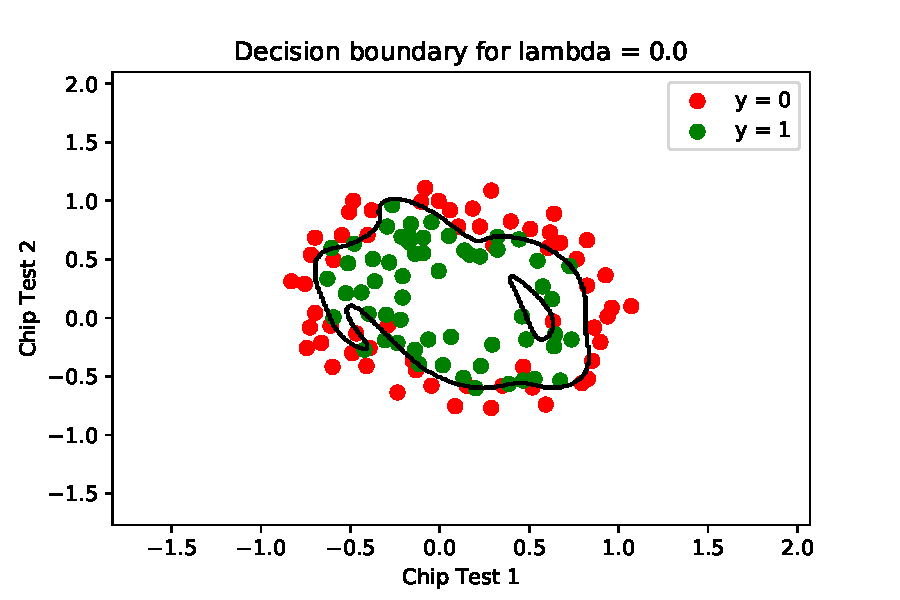
\includegraphics[scale=0.5]{fig4_overfit}
\end{center}
Underfit ($\lambda = 100$)
\begin{center}
	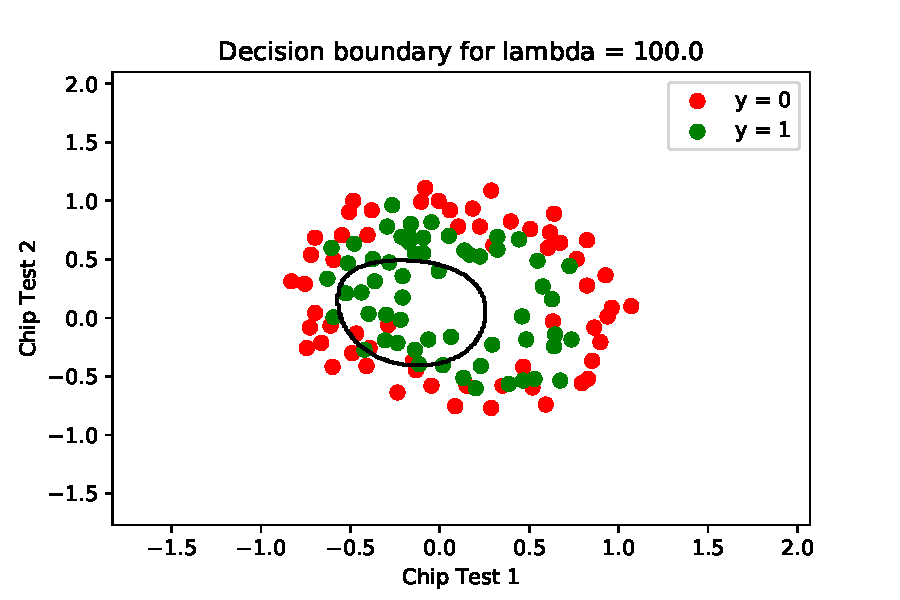
\includegraphics[scale=0.5]{fig4_underfit}
\end{center}


\subsection*{Problem 3B4: Exploring L1 and L2 penalized logistic regression}
From the results below, we can see that when $\lambda$ is small, loss of L2 > loss of L1; when $\lambda$ is large, loss of L2 < loss of L1. For both L1 and L2, loss increases as $\lambda$ increases.
L2 usually does not have exactly 0 parameters, while for L1, as $\lambda$ increases, the number of 0 parameters increases.\\
Loss value for L1 and L2 penalized logistic regression models with varying $\lambda$
\begin{center}
\begin{tabular}{ c c c c}
  &  $\lambda = 0.01 $& $\lambda = 1$& $\lambda = 3$\\ 
L1 & 0.291099818231 & 0.438147596196 & 0.613731793543 \\  
L2 & 0.316699562017 & 0.46843403006 & 0.549552378642  
\end{tabular}
\end{center}
L1 Regularization Path
\begin{center}
	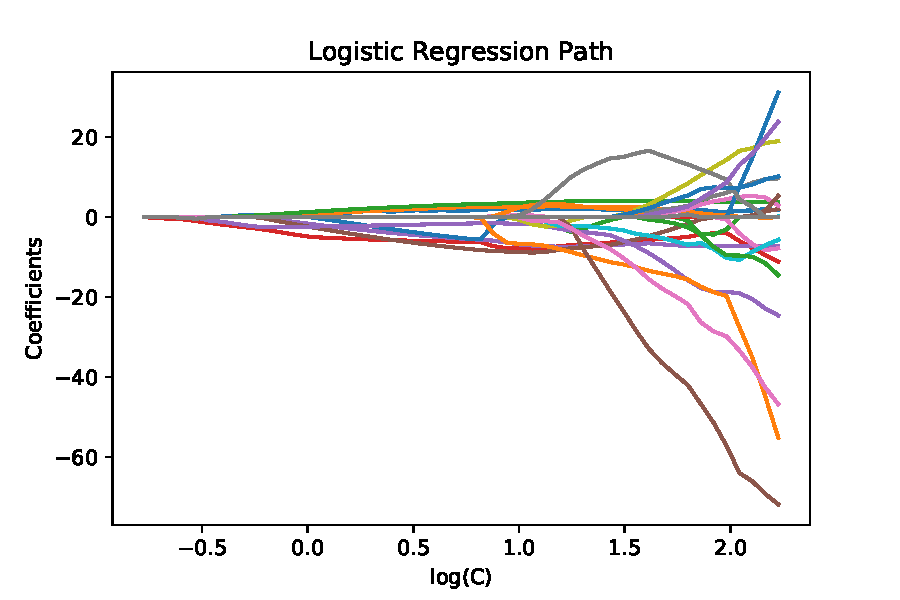
\includegraphics[scale=0.5]{fig5}
\end{center}
Number of non-zero parameters for L1 and L2 penalized logistic regression models with varying $\lambda$\\[0.5cm]
When $\lambda = 0.01 $:\\
Theta found by sklearn with L1 reg:  [  3.14107860e+00   3.20194249e-01   3.81520546e+00  -3.91738906e+00
  -7.20371638e+00   0.00000000e+00   4.64621488e+00   6.38109343e+00
   1.50107064e+01   0.00000000e+00   6.20675798e-04   0.00000000e+00
  -2.63197403e+00   0.00000000e+00  -1.85927659e+01   0.00000000e+00
  -8.99239588e-01   8.86292141e+00   0.00000000e+00  -1.12114255e+01
   7.15637196e+00  -2.00413010e+01  -1.00945038e+01   0.00000000e+00
   9.14366563e+00  -5.90473809e+01  -2.99446453e+01   0.00000000e+00]\\
Theta found by sklearn with L2 reg:  [ 3.74522253  2.0107989   4.61214155 -5.45414606 -6.67189659 -5.94010197
  2.151067   -0.10213815  2.45921341 -2.5147764  -3.80255072  2.98381388
 -3.77718734 -1.96294588 -6.31923347 -1.71938626 -0.86707608  4.99914053
 -3.62305722 -4.32524672  2.8515795  -5.47204508  0.45198499 -0.88342842
  3.20815872 -4.5010269  -3.62599862  0.26743958]\\[0.5cm]
When $\lambda = 1 $:\\
Theta found by sklearn with L1 reg:  [ 1.86967059  0.68660464  1.28039276 -4.8626065  -1.62174342 -2.34232494
  0.          0.          0.          0.          0.          0.          0.
  0.         -2.36735173  0.          0.          0.          0.          0.
  0.          0.          0.          0.          0.          0.          0.
  0.        ]\\
Theta found by sklearn with L2 reg:  [ 1.1421394   0.60141117  1.16712554 -1.87160974 -0.91574144 -1.26966693
  0.12658629 -0.3686536  -0.34511687 -0.17368655 -1.42387465 -0.04870064
 -0.60646669 -0.26935562 -1.16303832 -0.24327026 -0.20702143 -0.04326335
 -0.28028058 -0.286921   -0.46908732 -1.03633961  0.02914775 -0.29263743
  0.01728096 -0.32898422 -0.13801971 -0.93196832]\\[0.5cm]
When $\lambda = 3 $:\\
Theta found by sklearn with L1 reg:  [ 0.32973525  0.          0.         -1.3745988   0.          0.          0.
  0.          0.          0.          0.          0.          0.          0.
 -0.76898728  0.          0.          0.          0.          0.          0.
  0.          0.          0.          0.          0.          0.          0.        ]\\
 Theta found by sklearn with L2 reg:  [  5.89106253e-01   1.95454002e-01   5.58913807e-01  -9.86107898e-01
  -3.61900628e-01  -5.82750147e-01  -2.51639321e-02  -1.58019487e-01
  -1.59981994e-01  -1.45612675e-01  -7.58932186e-01  -3.41689773e-02
  -2.88651654e-01  -9.74950793e-02  -6.16273324e-01  -1.80925636e-01
  -9.79992358e-02  -4.05896085e-02  -1.27023699e-01  -1.16537109e-01
  -3.39110258e-01  -5.60445739e-01   5.57877067e-05  -1.43900969e-01
   5.69591879e-04  -1.57722446e-01  -4.39086378e-02  -5.60735202e-01]\\[0.5cm]
   

\subsection*{Problem 3 Part C: Logistic regression for spam classification}
L1 models are in general very sparse while L2 models are not sparse. The results also show that the binarize L1 model is not sparse compared to the other L2 models.\\[0.5cm]
According to the accuracy scores shown in the table below, L1 and L2 have very similar accuracy for the given data set. However, since L1 models are in general sparse, they usually have fewer non-zero parameters than L2 models. Considering we have 57 features in the data set, we may prefer to have a model with only the most important features to make predictions. In that case, I would recommend L1 regularization.\\[0.5cm]
Accuracy for L1 and L2 penalized logistic regression models with different data scaling methods
\begin{center}
\begin{tabular}{ c c c c}
  &  Standardization & Log Transformation & Binarization\\ 
L1 & 0.923828125 & 0.944010416667 & 0.92578125 \\  
L2 & 0.921875 & 0.943359375 &  0.928385416667  
\end{tabular}
\end{center}






\end{document}



